\documentclass[runningheads]{llncs}
\usepackage[T1]{fontenc}
\usepackage{graphicx}
\usepackage{booktabs}
\usepackage{multirow}
\usepackage{amsmath}
\usepackage{url}
\usepackage{float}
\usepackage[hidelinks]{hyperref}
\usepackage[section]{placeins}
\graphicspath{{figures/}}
\pagestyle{plain}
\raggedbottom
\setlength{\textfloatsep}{10pt plus 2pt minus 2pt}
\setlength{\floatsep}{8pt plus 2pt minus 2pt}
\setlength{\intextsep}{8pt plus 2pt minus 2pt}
\setlength{\abovecaptionskip}{6pt}
\setlength{\belowcaptionskip}{2pt}
\begin{document}

\title{PlasmaXAI: Counterfactual-Guided Explainable Fusion for Malignant Plasma Cell Recognition and Patient-Level Morphologic Consistency Analysis}
\titlerunning{PlasmaXAI}
\author{Arnob Aich Anurag}
\institute{American International University-Bangladesh, Dhaka, Bangladesh}
\authorrunning{Anurag et al.}

\maketitle
\thispagestyle{plain}

\begin{abstract}
Reliable plasma cell assessment is central to multiple myeloma diagnosis, yet manual microscopic review is labor-intensive and difficult to scale in resource-constrained laboratories. This paper presents PlasmaXAI, an explainable computational pathology framework for malignant plasma cell recognition. PlasmaXAI combines frozen ResNet50 and DenseNet121 image embeddings with handcrafted morphology, a morphology-derived counterfactual boundary model, and a learned gating mechanism that injects counterfactual signals directly into the decision path. Evaluated on PCMMD, PlasmaXAI achieves 93.42\% accuracy, 93.43\% weighted F1, 91.24\% plasma precision, 94.63\% plasma recall, and 97.76\% AUC at the selected precision-recall balanced operating point. Beyond classification, the framework provides counterfactual analysis, calibration and bootstrap summaries, ablation evidence, and exploratory patient-level robustness results. The study positions PlasmaXAI as a practical explainable screening framework for digital hematopathology workflows that need both performance and transparent reasoning.
\keywords{Multiple myeloma \and Digital pathology \and Explainable AI \and Counterfactual analysis \and Plasma cell recognition \and Deep learning}
\end{abstract}

\section{Introduction}
Multiple myeloma remains a clinically important hematologic malignancy in which plasma cell morphology plays a major role in screening, diagnosis, and treatment monitoring \cite{mmreview}. In practice, plasma cell assessment often depends on manual microscopic review of stained bone marrow smears, where inter-observer variability, fatigue, stain variability, and high case volume can all reduce consistency. These challenges are especially relevant in low-resource settings where specialist review time is limited.

Deep learning has demonstrated strong value in medical image analysis and digital pathology, but high raw performance alone is insufficient \cite{litjens,bera,campanella}. A clinically useful plasma-cell model should also expose the evidence behind its prediction so that its behavior can be trusted, calibrated, and audited.

PlasmaXAI is designed around that premise. It integrates counterfactual morphology signals directly into a learned fusion model that combines image representation, handcrafted morphology, boundary distance, and modality gating. This paper contributes an explainable multi-branch plasma cell classifier, a counterfactual-aware decision path, and an evaluation protocol that includes calibration, bootstrap uncertainty, ablation analysis, and patient-level robustness.

\section{Literature Review}
Convolutional neural networks dominate modern medical image analysis because they learn hierarchical features more effectively than handcrafted descriptors alone \cite{litjens,janowczyk}. In digital pathology, clinically useful models must balance local texture sensitivity with stable higher-level semantics \cite{bera,campanella}. Residual networks improve optimization through identity mapping, while densely connected networks promote feature reuse and stronger gradient flow \cite{resnet,densenet}. Encoder-decoder models such as U-Net and attention-augmented variants show how feature fusion can improve biomedical visual reasoning \cite{unet,attentionunet}. These backbones are attractive for plasma cell morphology because they capture complementary structural and chromatic cues.

Pathology tasks also differ from generic natural-image classification. Cellular boundaries, stain intensity, nucleus-to-cytoplasm ratio, and chromatic variation can all be clinically meaningful. This has motivated hybrid systems that combine learned image embeddings with structured morphology features.

Explainable AI methods are commonly divided into post-hoc attribution, local surrogate explanation, saliency-based visualization, and counterfactual reasoning \cite{lime,gradcam,shap,wachter}. Counterfactual explanations are especially valuable in healthcare because they answer a clinically intuitive question: what minimal feature changes would move a prediction toward a different outcome? Wachter et al. formalized counterfactual explanation as a practical way to interrogate automated decisions without full model transparency \cite{wachter}, while DICE demonstrated how diverse counterfactual sets can support actionable model interpretation \cite{diceml}. Calibration analysis is also critical because high-confidence predictions are only useful if they correspond to observed outcome frequencies \cite{calibration}.

PlasmaXAI builds on these directions by treating counterfactual information as part of the model input rather than only the model output. The framework therefore occupies a middle ground between black-box classification and purely descriptive explainability, allowing performance optimization and interpretability to reinforce each other.

\section{Materials and Methods}
\subsection{Dataset and Feature Construction}
The study uses PCMMD cell images organized into a cell-level training split and a separate patient-organized cohort for exploratory patient analysis. Each cell image is resized to 224 $\times$ 224 and normalized for CNN feature extraction. In parallel, a morphology pipeline computes nucleus-to-cytoplasm ratio, nucleus area, cytoplasm area, staining intensity, granularity, roundness, and mean RGB channels. These descriptors provide an interpretable phenotype layer that complements the learned visual embeddings.

\subsection{PlasmaXAI Architecture}
PlasmaXAI combines two frozen image backbones, ResNet50 and DenseNet121, with morphology, counterfactual, and score branches. A logistic morphology model first estimates a counterfactual boundary that separates plasma and non-plasma behavior in the handcrafted feature space. From that boundary, the framework derives feature-shift and distance terms describing how a sample would need to change in order to move toward the benign decision region.

These counterfactual features are then passed into a learned fusion model. Separate encoders process the ResNet, DenseNet, morphology, counterfactual, and score streams. Counterfactual signals modulate the image features through sigmoid gates, refine the score branch, and contribute to a softmax modality gate that controls the final fusion weights. This design makes the counterfactual pathway structurally important rather than decorative. The overall framework is shown in Fig.~\ref{fig:framework}, while a more detailed block-level architecture is shown in Fig.~\ref{fig:archdetail}.

\begin{figure}[!htbp]
\centering
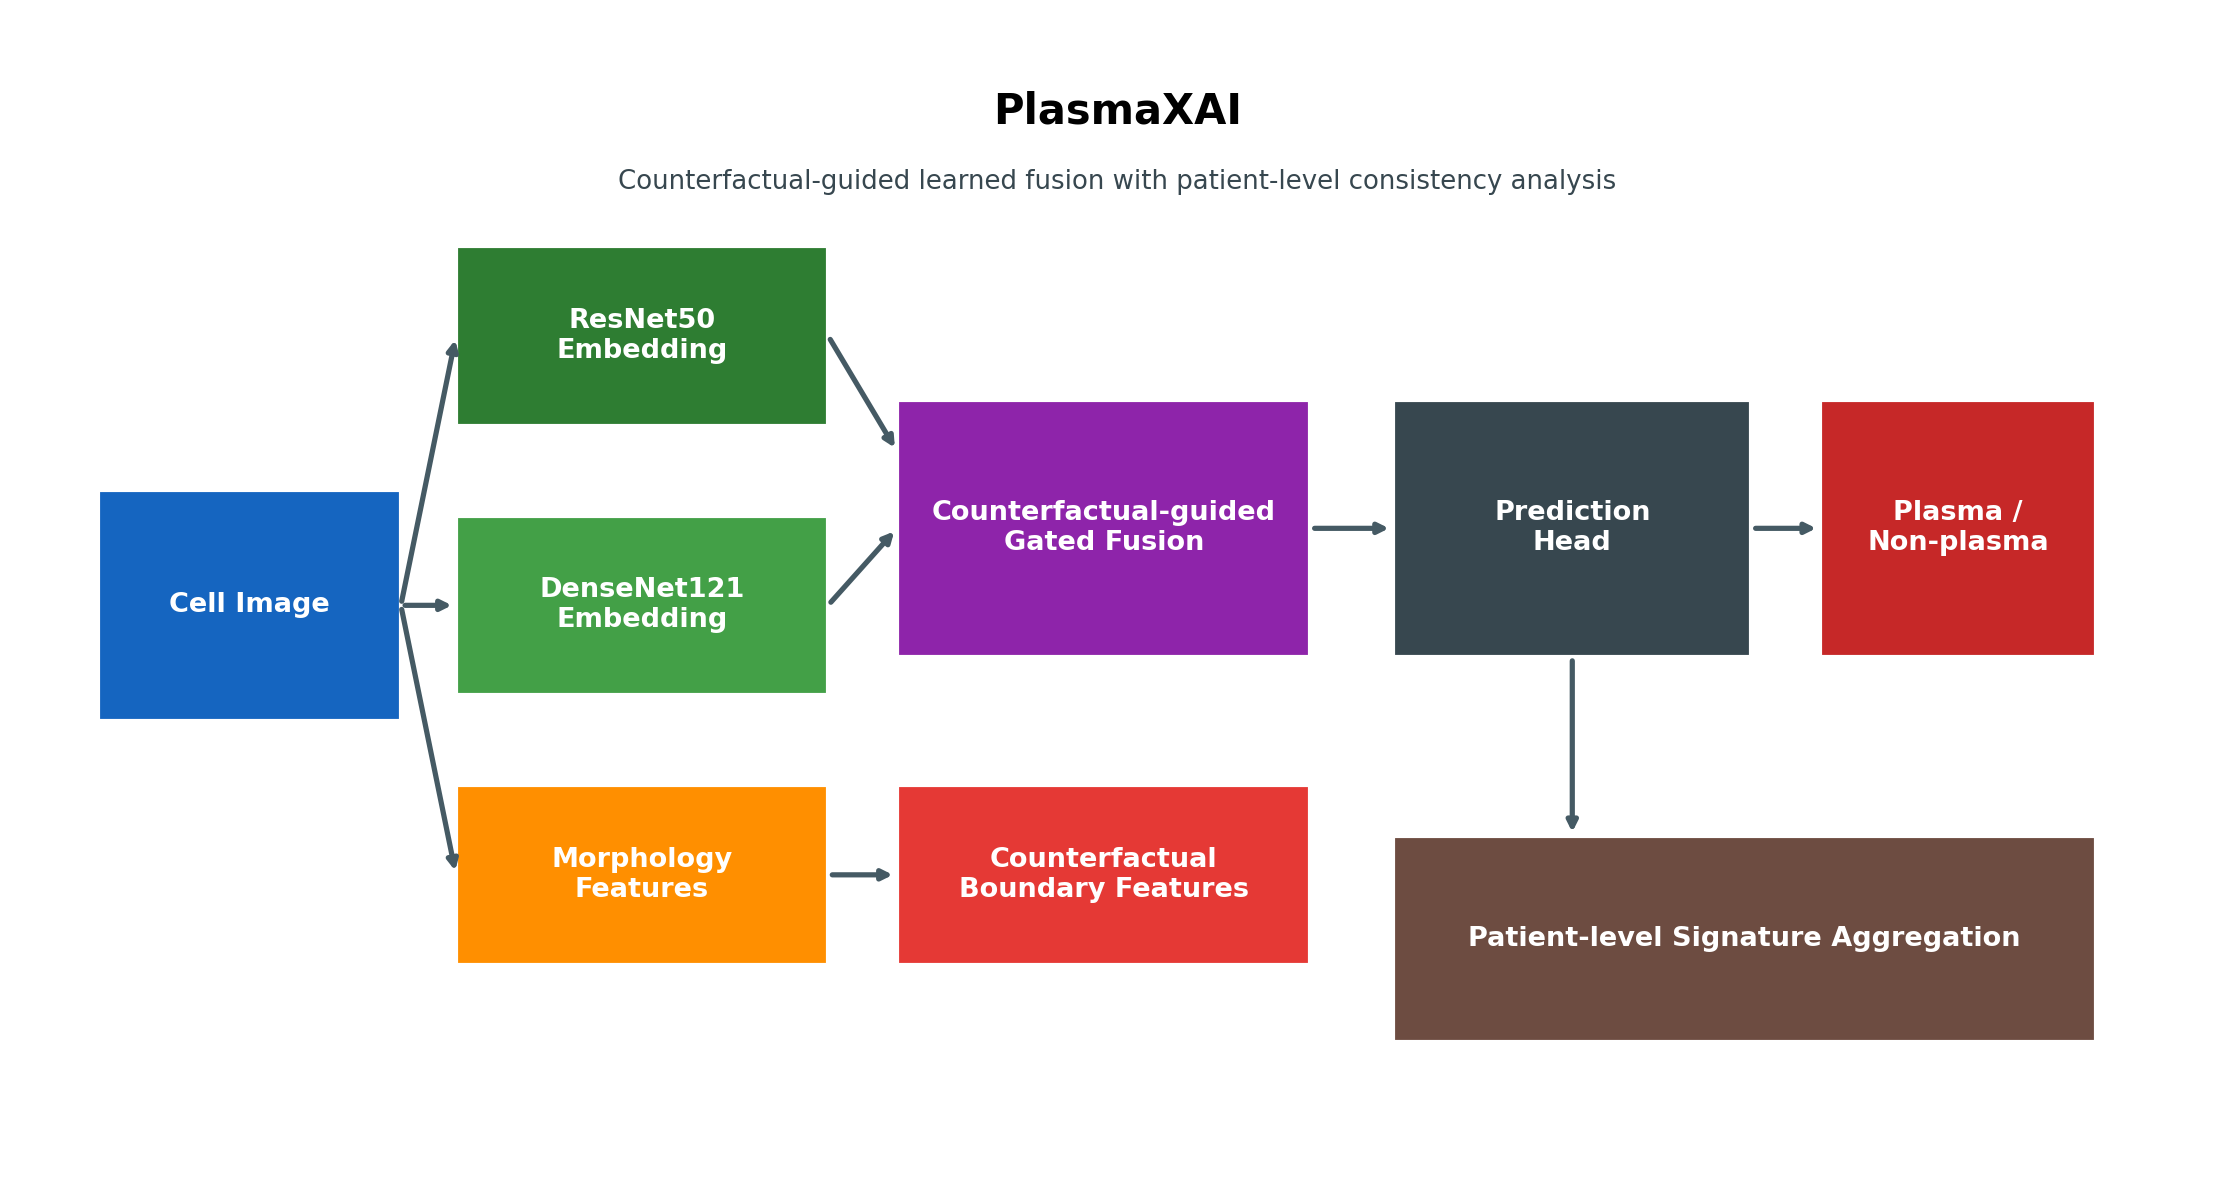
\includegraphics[width=0.94\textwidth]{plasmaxai_framework.png}
\caption{PlasmaXAI framework showing image embeddings, morphology features, counterfactual-guided fusion, and explainability outputs.}
\label{fig:framework}
\end{figure}
\begin{figure}[!htbp]
\centering
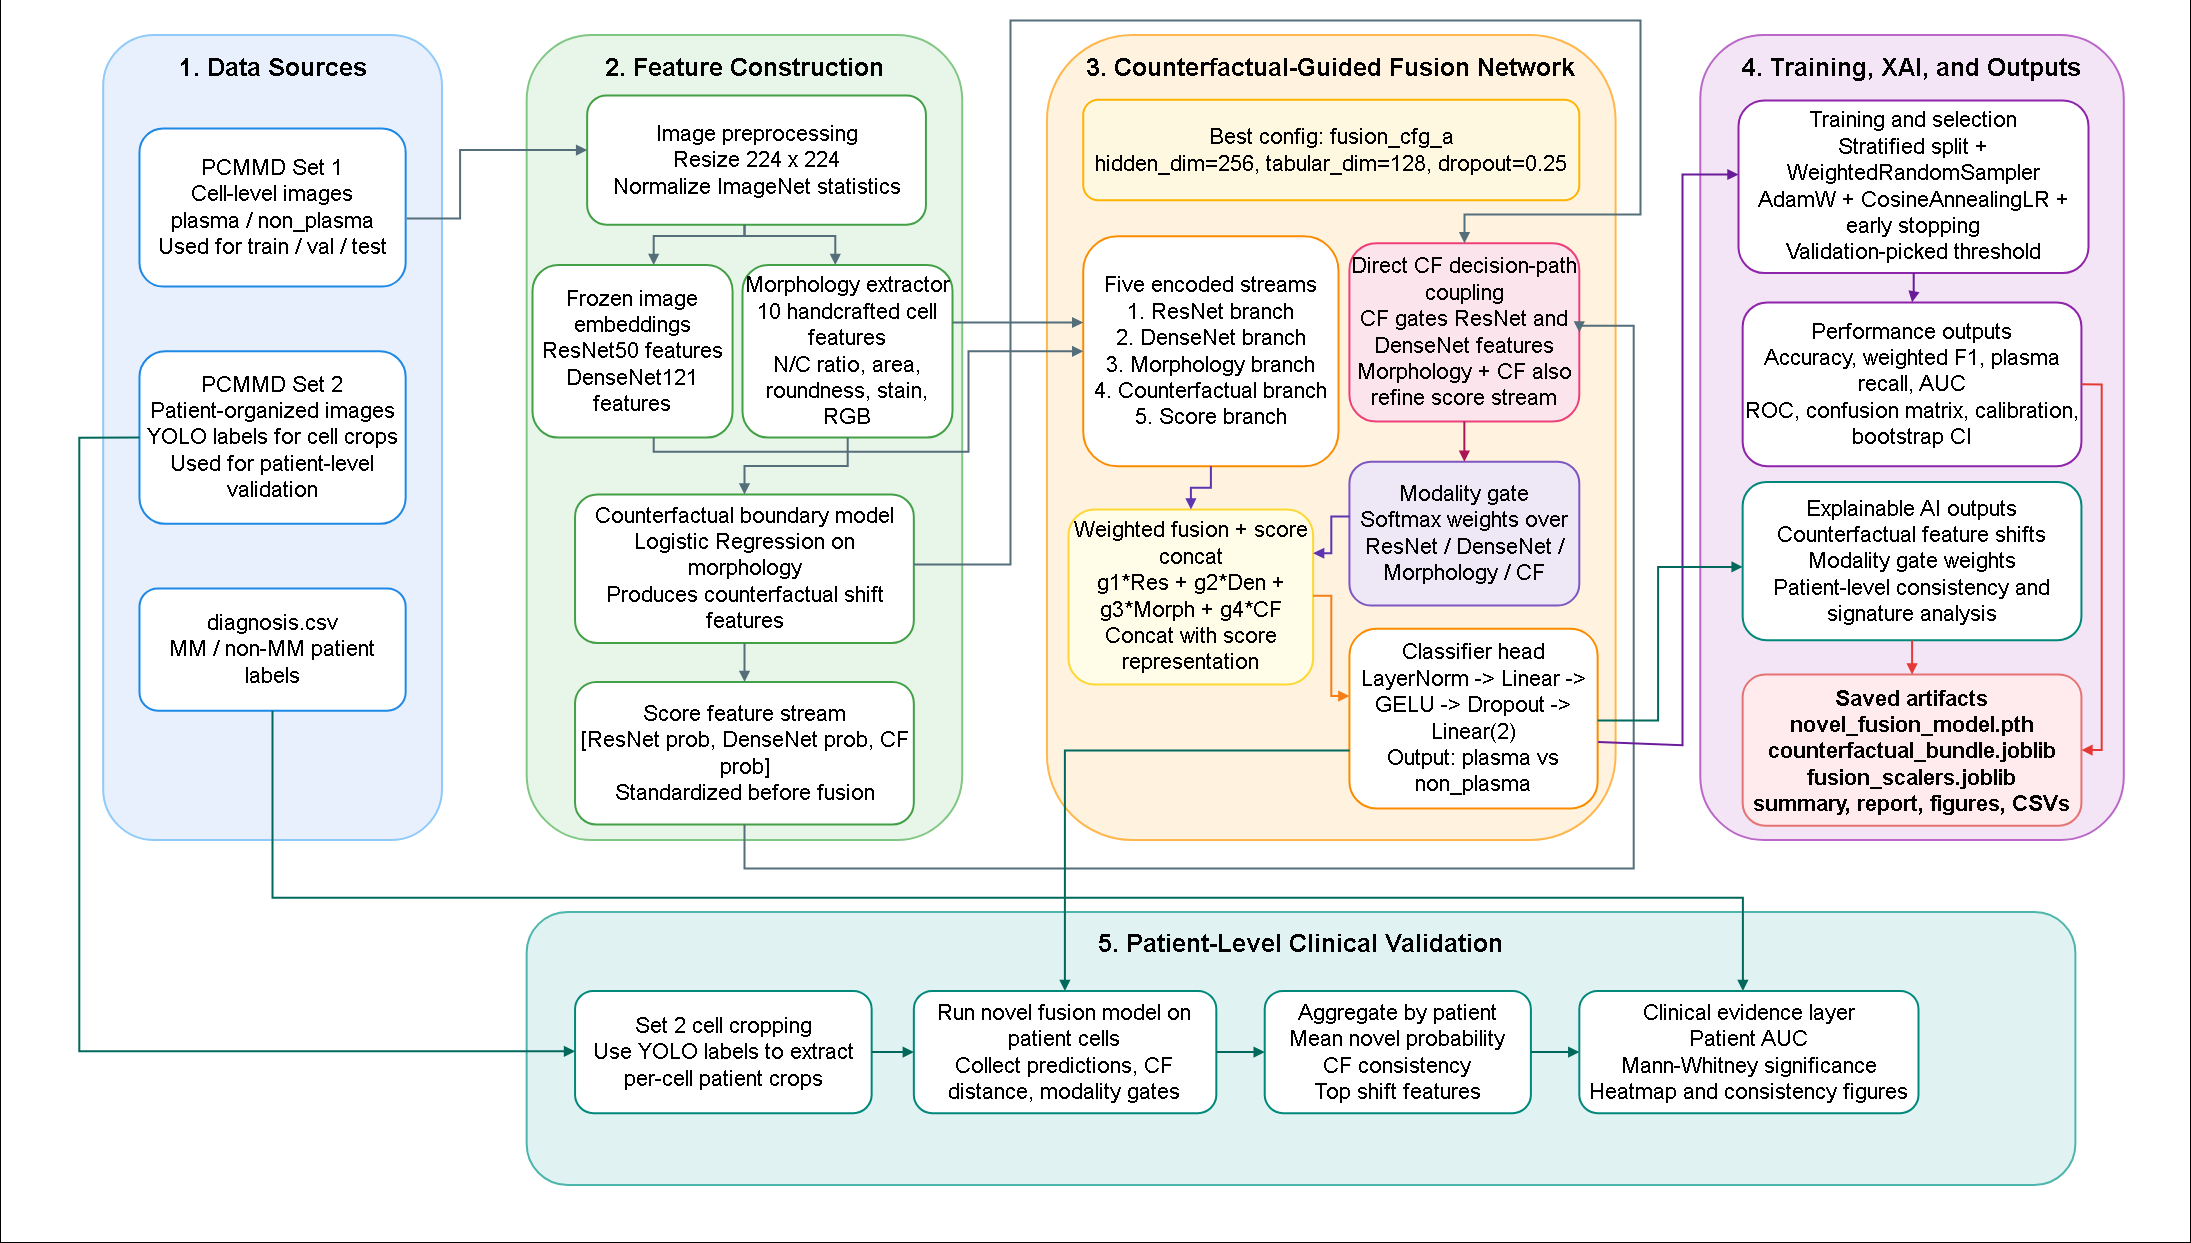
\includegraphics[width=0.88\textwidth]{Architecture_diagram.png}
\caption{Detailed PlasmaXAI architecture diagram highlighting the internal fusion blocks and information flow.}
\label{fig:archdetail}
\end{figure}
Figure~\ref{fig:archdetail} details the internal fusion blocks and information flow.

\subsection{Evaluation Protocol}
The primary deployment operating point is the precision-recall balanced threshold selected on validation data. Final evaluation reports accuracy, weighted F1, plasma precision, plasma recall, and AUC, together with calibration curves, bootstrap confidence intervals, ablation variants, and patient-level robustness checks based on exact permutation testing and leave-one-patient-out analysis.
\FloatBarrier

\section{Results and Discussion}
\subsection{Core Classification Results}
At the selected operating point, PlasmaXAI achieved 93.42\% accuracy, 93.43\% weighted F1, 91.24\% plasma precision, 94.63\% plasma recall, and 97.76\% AUC. It outperformed the strongest non-PlasmaXAI baselines on accuracy, precision, and recall. Table~\ref{tab:mainresults} and Fig.~\ref{fig:modelcomp} summarize the benchmark.

\begin{table}[!htbp]
\centering
\caption{Held-out test performance for the strongest comparison models.}
\label{tab:mainresults}
\begin{tabular}{lccccc}
\toprule
Model & Acc. (\%) & W-F1 (\%) & Prec. (\%) & Recall (\%) & AUC (\%) \\
\midrule
ResNet50 & 91.92 & 91.93 & 89.02 & 93.80 & 97.05 \\
Prev Hybrid & 91.73 & 91.73 & 90.91 & 90.91 & 97.12 \\
DenseNet121 & 89.85 & 89.83 & 90.17 & 87.19 & 96.36 \\
\textbf{PlasmaXAI} & \textbf{93.42} & \textbf{93.43} & \textbf{91.24} & \textbf{94.63} & \textbf{97.76} \\
\bottomrule
\end{tabular}
\end{table}
\begin{figure}[!htbp]
\centering
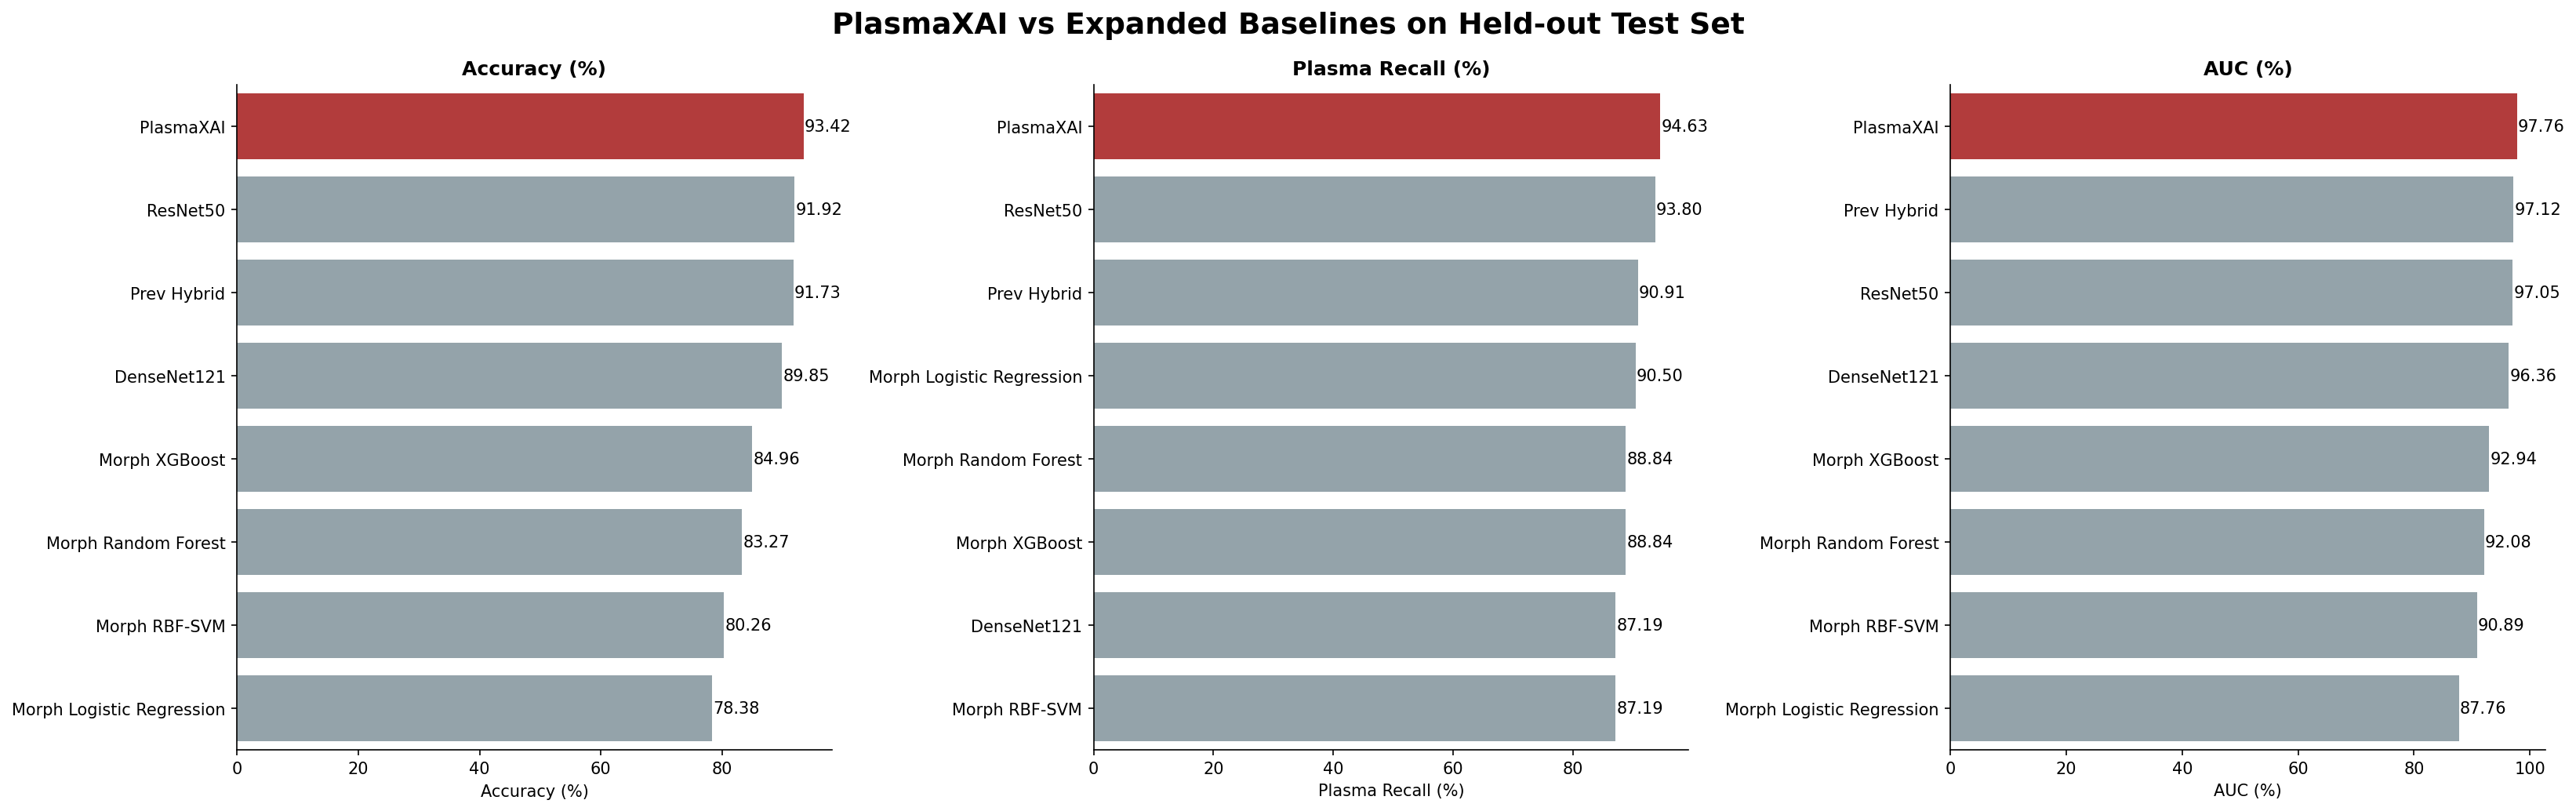
\includegraphics[width=0.95\textwidth]{plasmaxai_model_comparison.png}
\caption{Expanded benchmark comparison showing PlasmaXAI against deep and morphology-based baselines.}
\label{fig:modelcomp}
\end{figure}
Figure~\ref{fig:modelcomp} shows that the full framework leads across the main deployment-oriented metrics.

Bootstrap analysis indicated that the chosen operating point was stable, with a 95\% confidence interval of 91.16--95.30 for accuracy, 91.30--97.20 for plasma recall, and 96.56--98.63 for AUC. This matters because a clinically useful system must remain strong under resampling, not only at one favorable threshold.

\subsection{Explainability, Ablation, and Patient-Level Findings}
The explainability pathway is one of the most distinctive parts of PlasmaXAI. The counterfactual explanation analysis in Fig.~\ref{fig:counterfactual} shows that the model learns meaningful modality weights while highlighting the dominant counterfactual drivers in the decision path. In practice, this means the classifier can surface not just a malignancy score, but also which morphology shifts most influence that score.

\begin{figure}[!htbp]
\centering
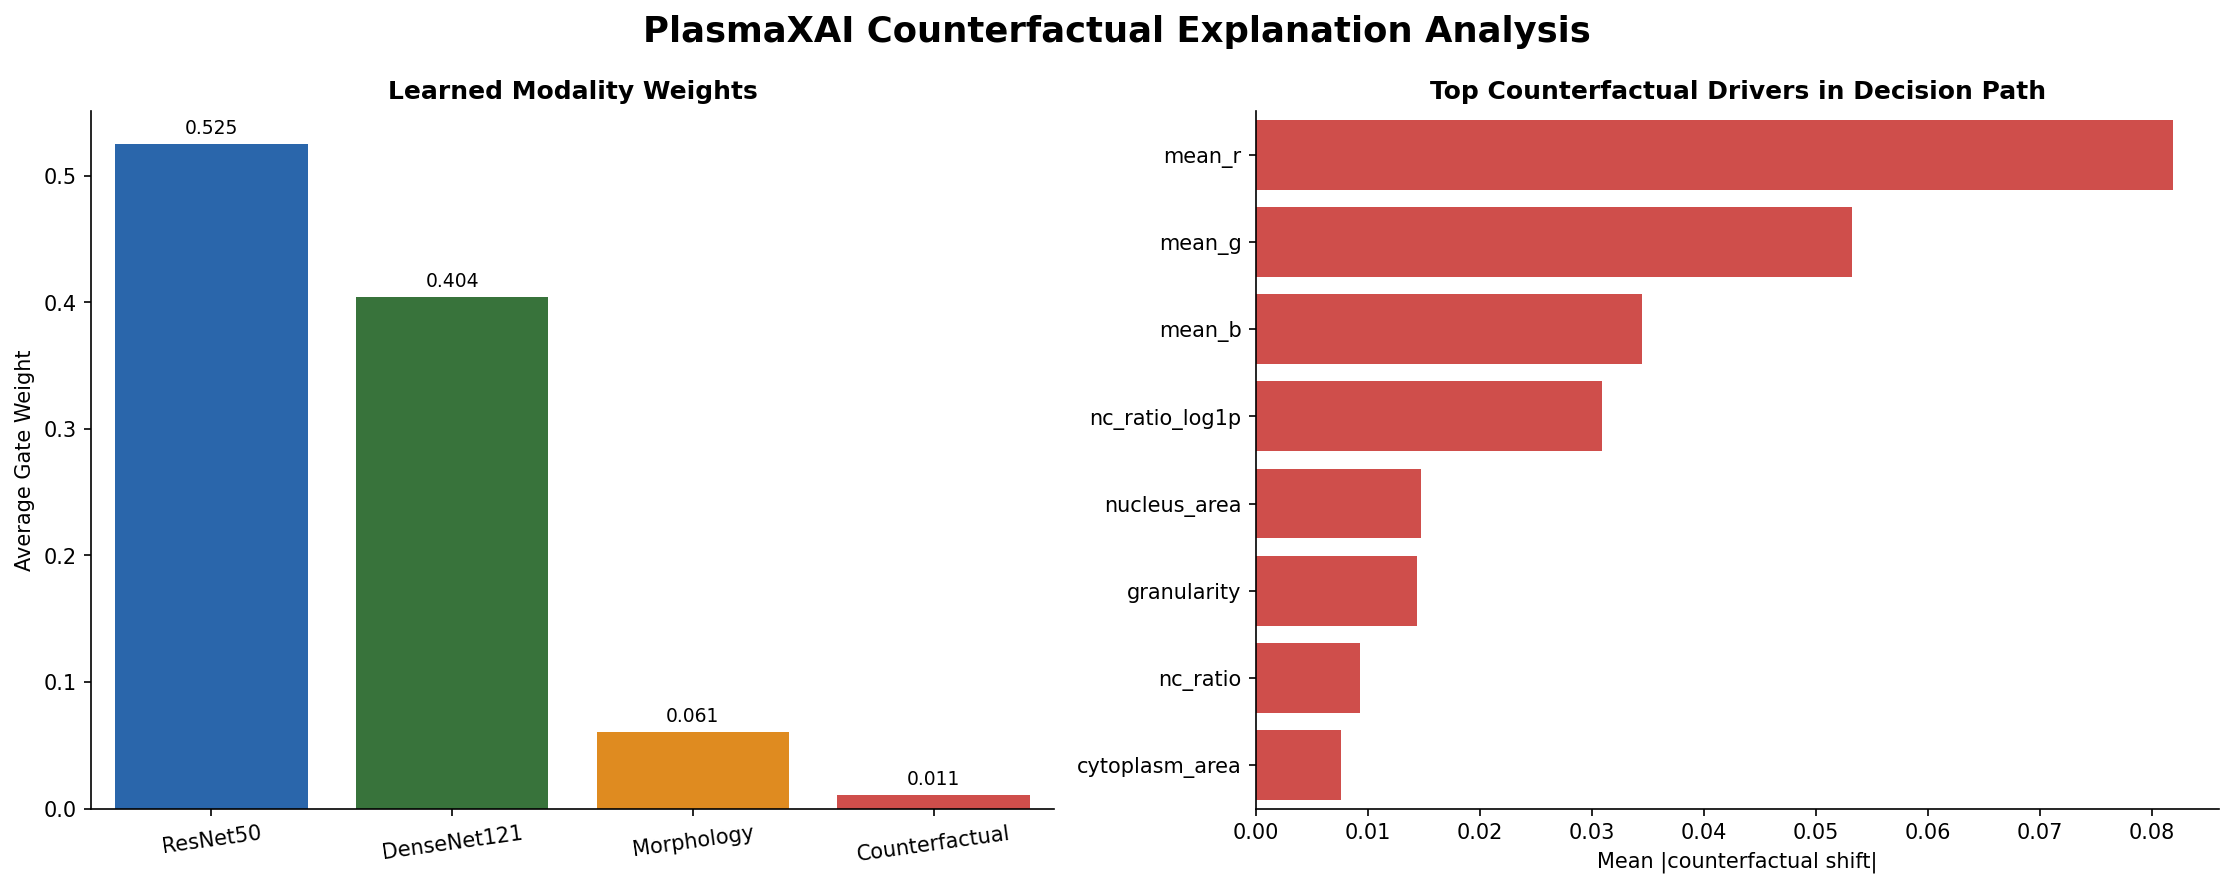
\includegraphics[width=0.95\textwidth]{plasmaxai_counterfactual.png}
\caption{Counterfactual explanation analysis showing learned modality weights and dominant feature shifts in the decision pathway.}
\label{fig:counterfactual}
\end{figure}
Figure~\ref{fig:counterfactual} shows that explainability in PlasmaXAI is part of the classifier logic rather than a detached post-hoc overlay.

The ablation study reinforces the importance of the explainability-aware design. Removing the counterfactual path caused the largest recall drop, down to 85.95\%, while the morphology branch also remained useful. This pattern suggests that the main benefit of PlasmaXAI is the interaction between image features and counterfactual morphology reasoning. The ablation overview is shown in Fig.~\ref{fig:ablation}.

\begin{figure}[!htbp]
\centering
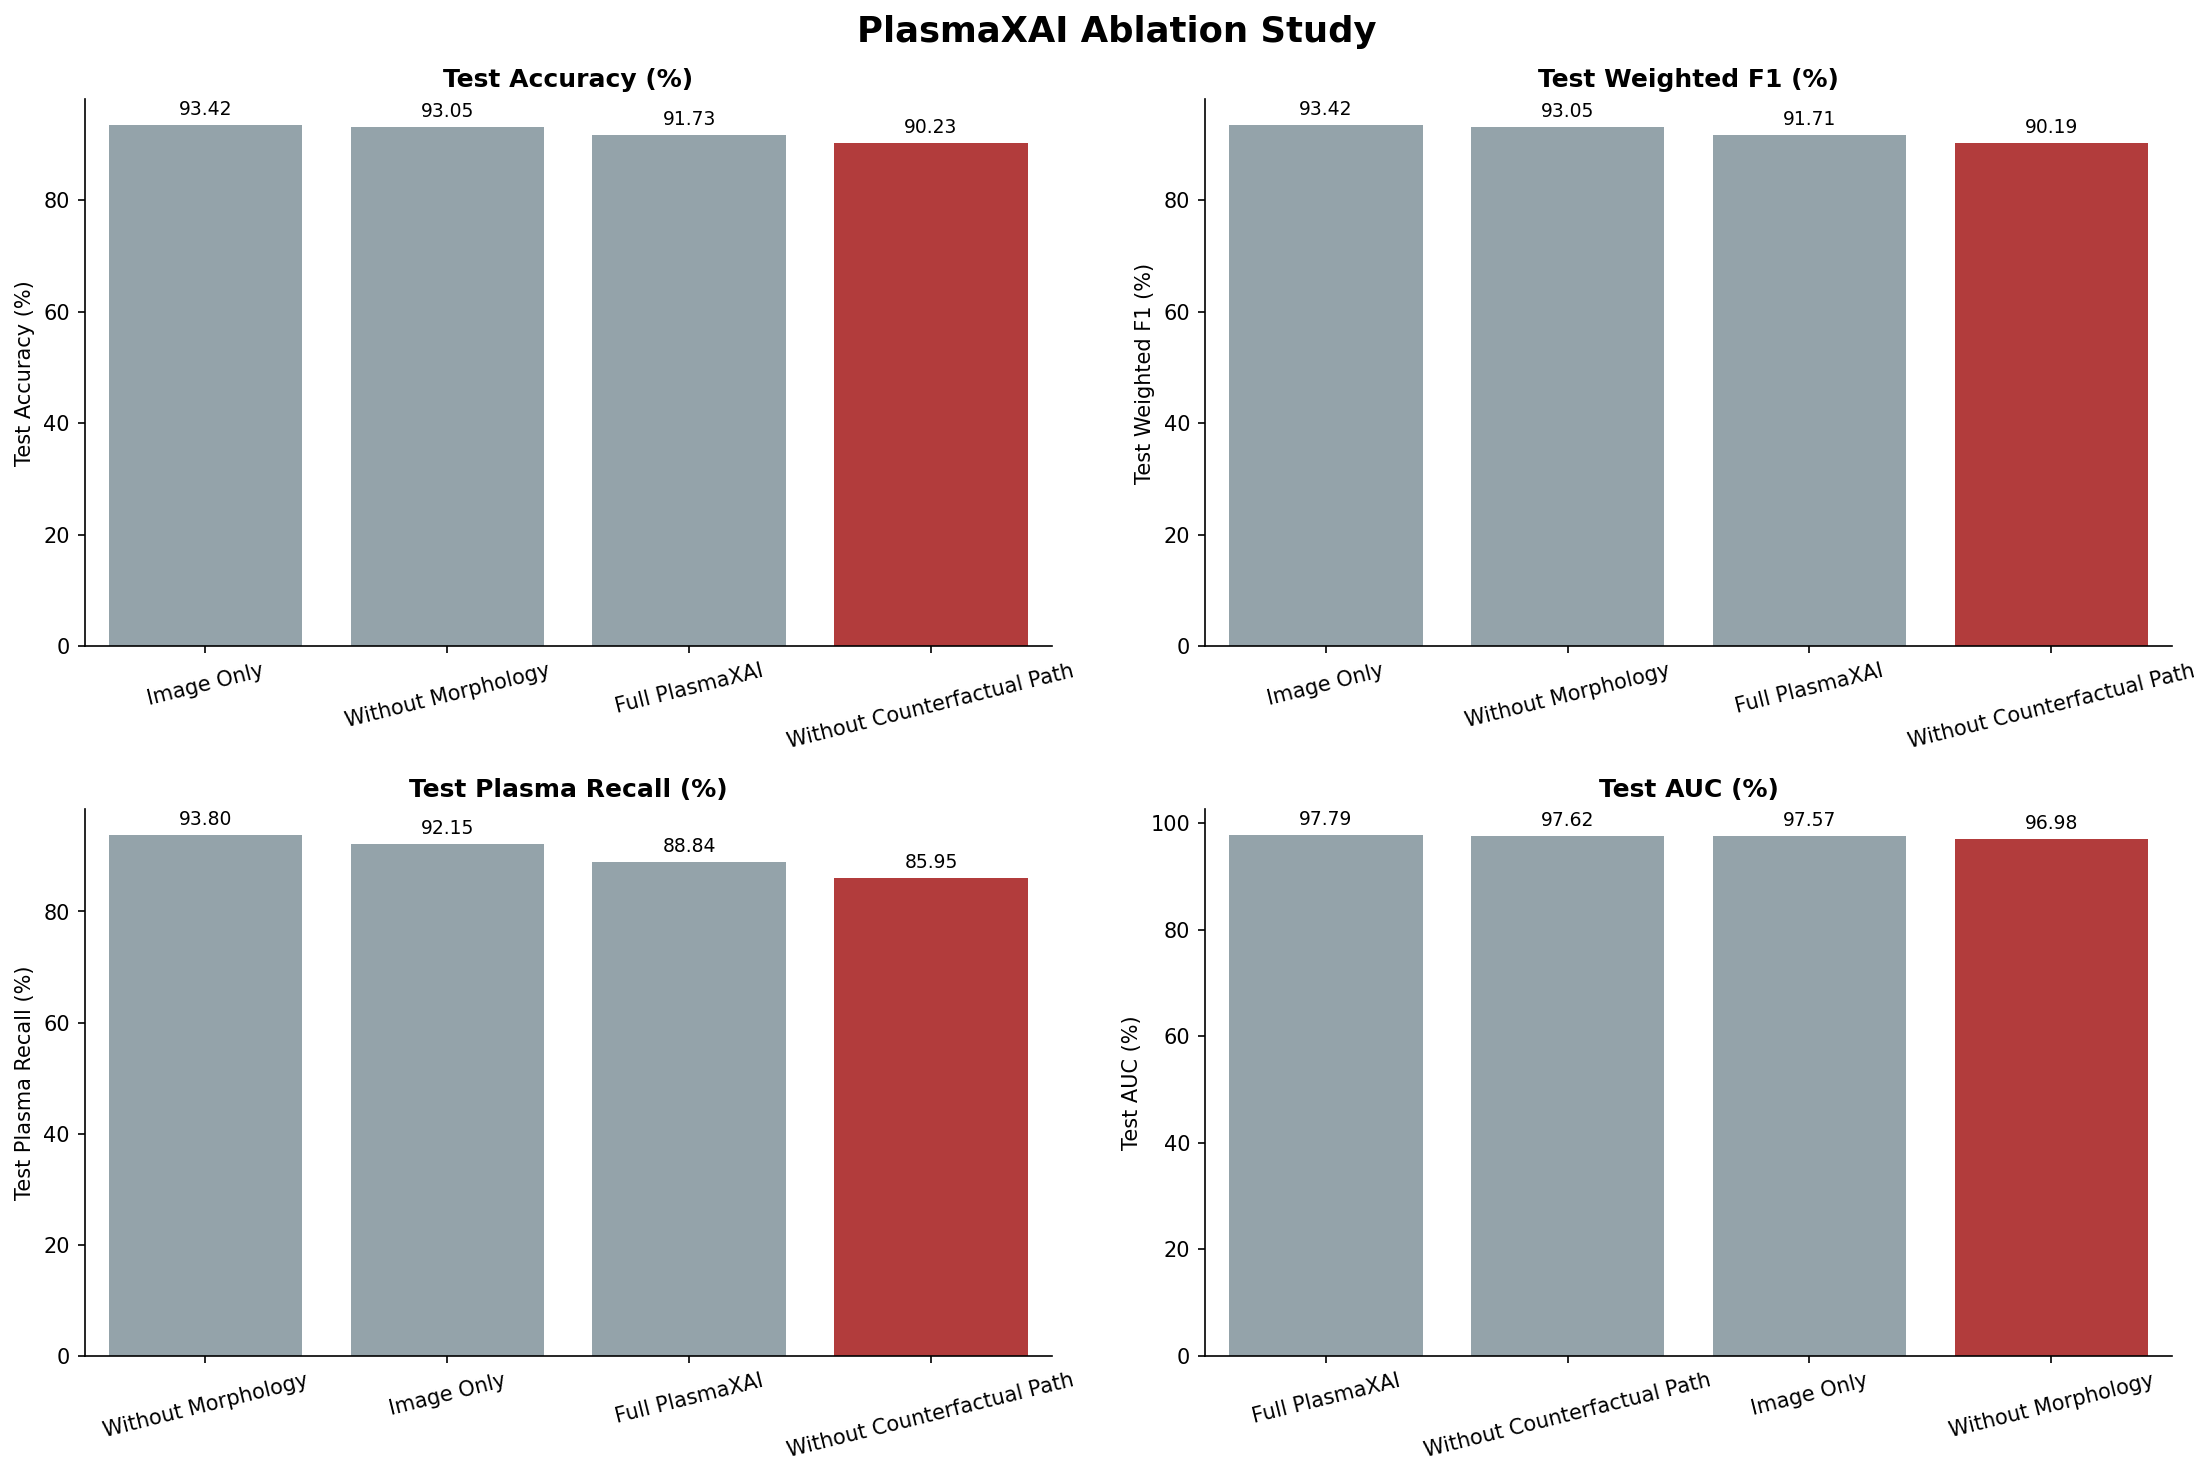
\includegraphics[width=0.95\textwidth]{plasmaxai_ablation.png}
\caption{Ablation study across image-only, no-morphology, no-counterfactual, and full PlasmaXAI variants.}
\label{fig:ablation}
\end{figure}
Figure~\ref{fig:ablation} confirms that the counterfactual branch contributes the most distinctive gain in malignant-cell sensitivity.

Patient-level analysis produced an internal AUC of 1.000 on a ten-patient cohort, with exact permutation p-values of 0.0040 one-sided and 0.0079 two-sided. This is encouraging, but it is not external clinical proof because the cohort is small and internally sourced. Figures~\ref{fig:calib}--\ref{fig:heatmap} therefore provide cautionary context for the otherwise strong internal separation.

\begin{figure}[!htbp]
\centering
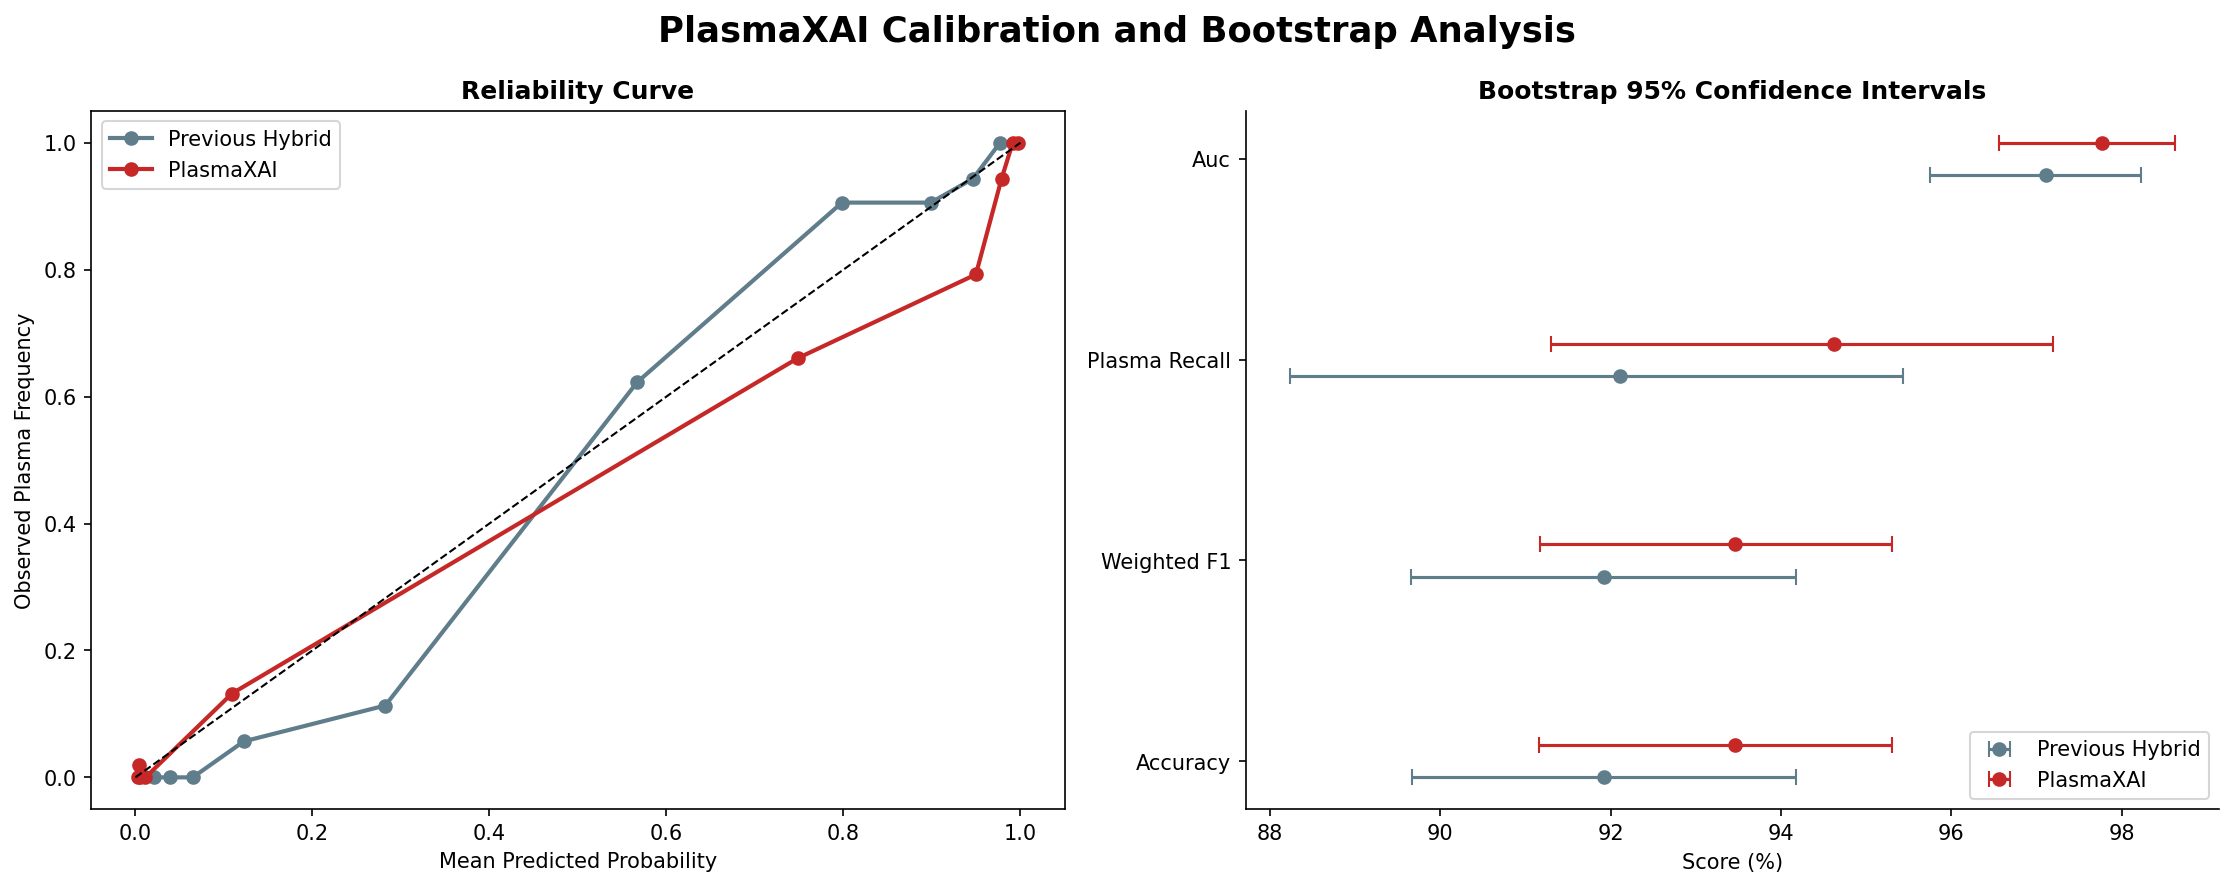
\includegraphics[width=0.95\textwidth]{plasmaxai_calibration_bootstrap.png}
\caption{Calibration and bootstrap-confidence analysis comparing PlasmaXAI with the previous hybrid model.}
\label{fig:calib}
\end{figure}
Figure~\ref{fig:calib} indicates that the selected operating point remains stable under resampling and is not driven by a single lucky split.

\begin{figure}[!htbp]
\centering
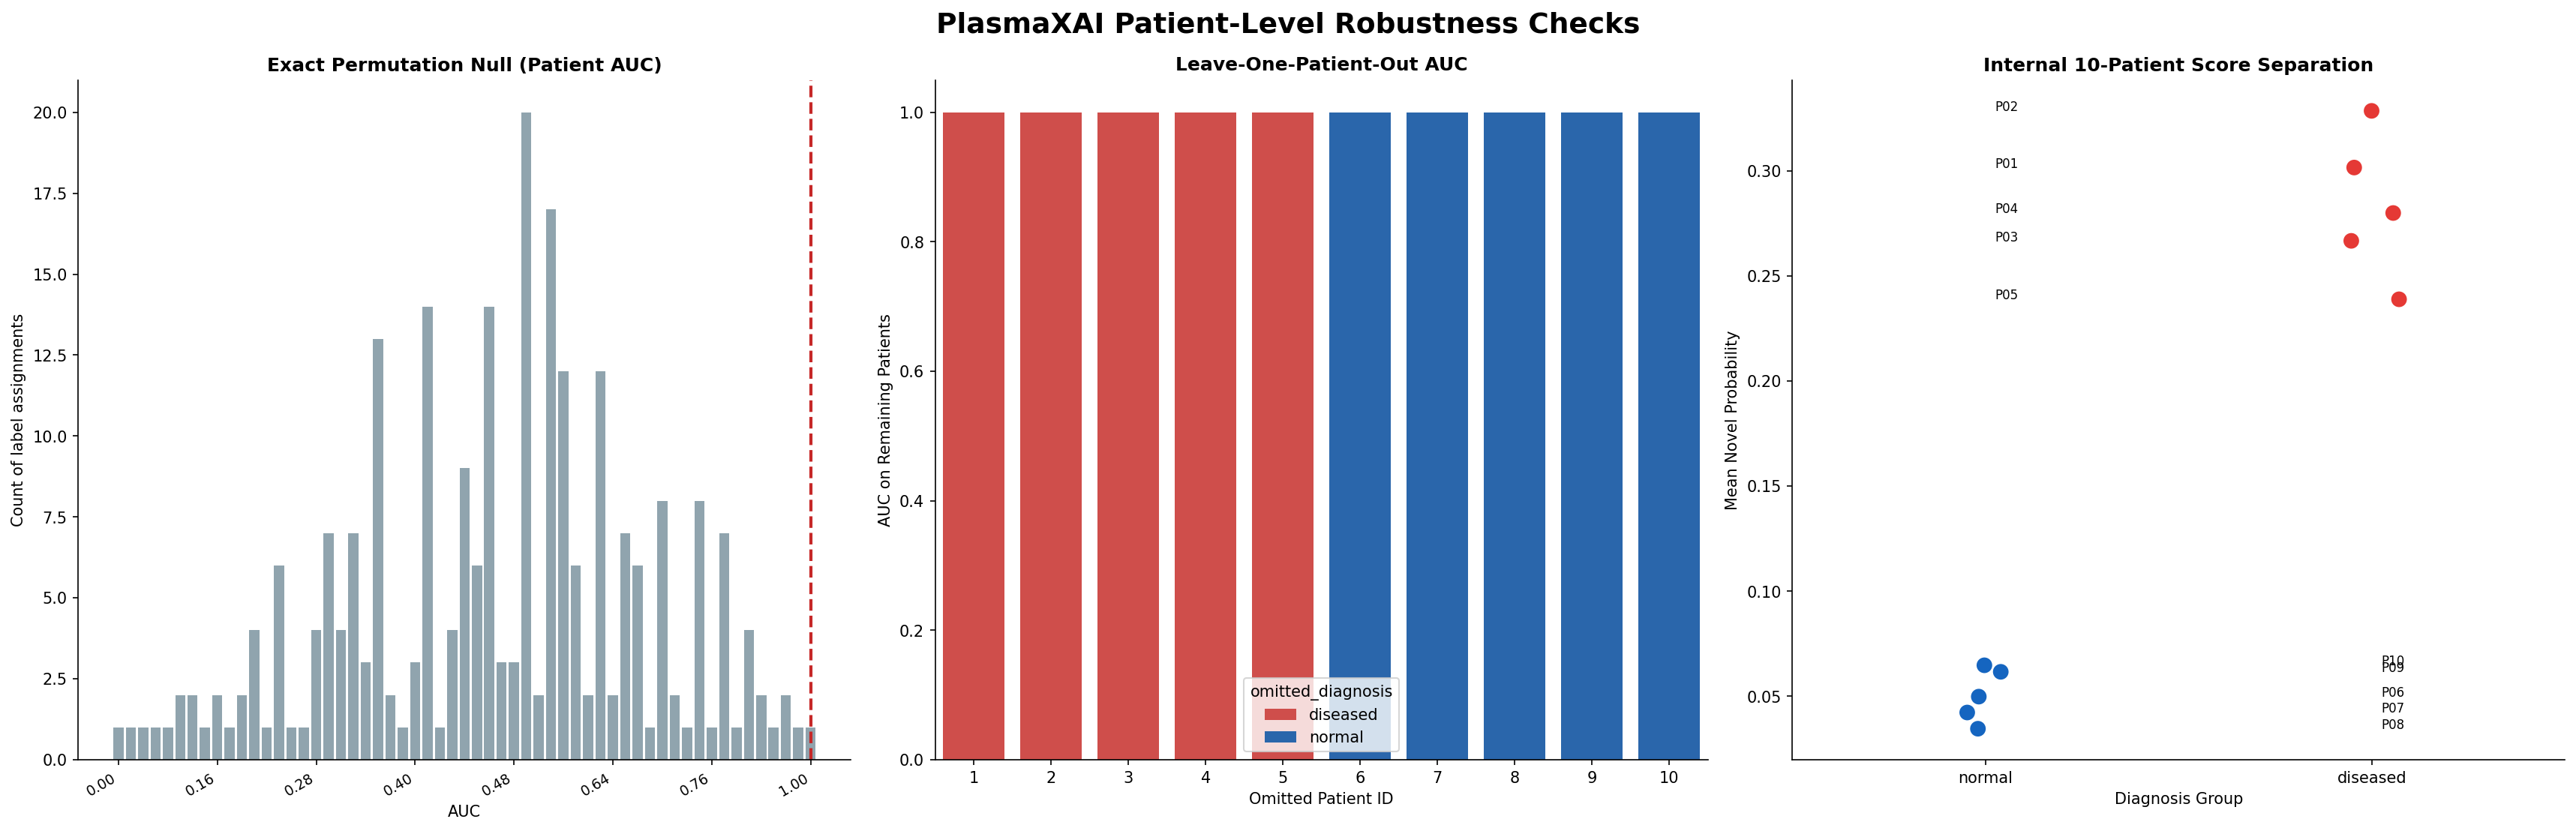
\includegraphics[width=0.95\textwidth]{plasmaxai_patient_robustness.png}
\caption{Patient-level robustness analysis with exact permutation null, leave-one-patient-out AUC, and score separation.}
\label{fig:patient}
\end{figure}
Figure~\ref{fig:patient} shows why the patient-level result still requires careful interpretation.

\begin{figure}[!htbp]
\centering
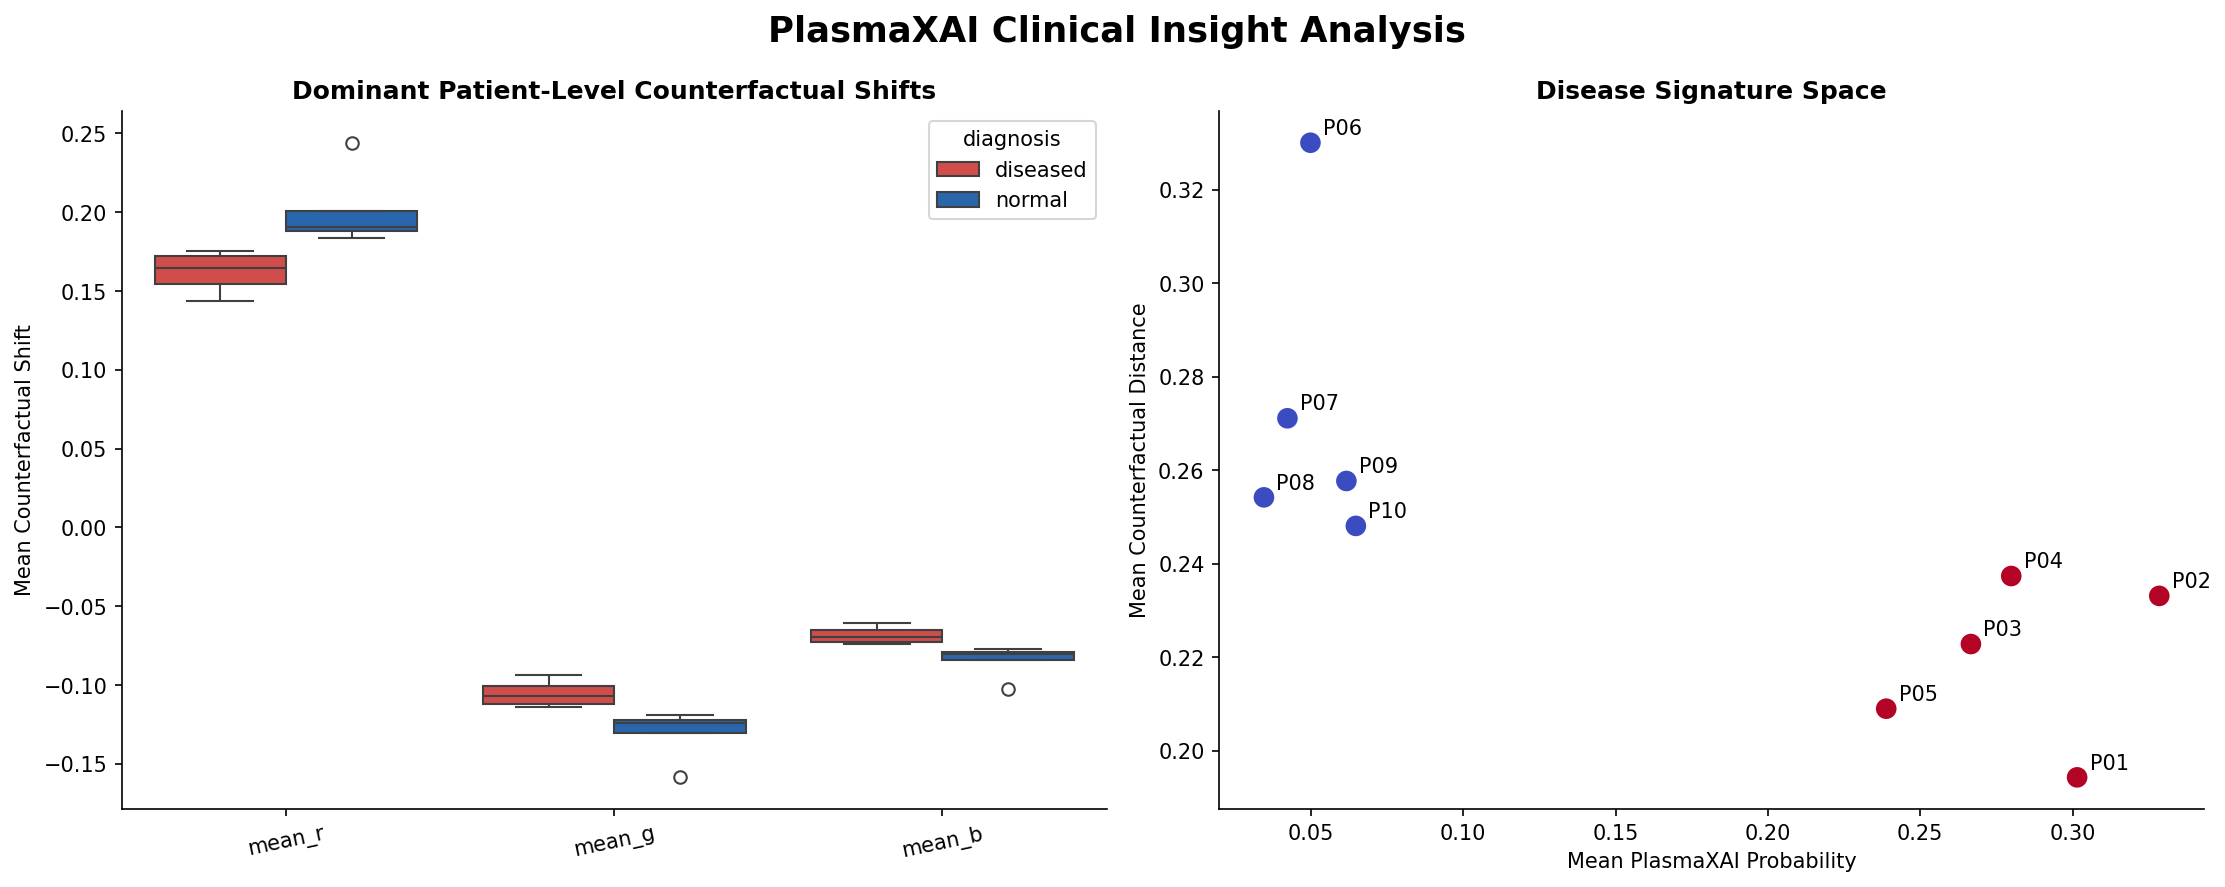
\includegraphics[width=0.95\textwidth]{plasmaxai_clinical_insight.png}
\caption{Clinical insight analysis showing dominant patient-level counterfactual shifts and disease-signature separation.}
\label{fig:clinical}
\end{figure}
Figure~\ref{fig:clinical} highlights the disease-signature space and the dominant feature shifts associated with the malignant cohort.

\begin{figure}[!htbp]
\centering
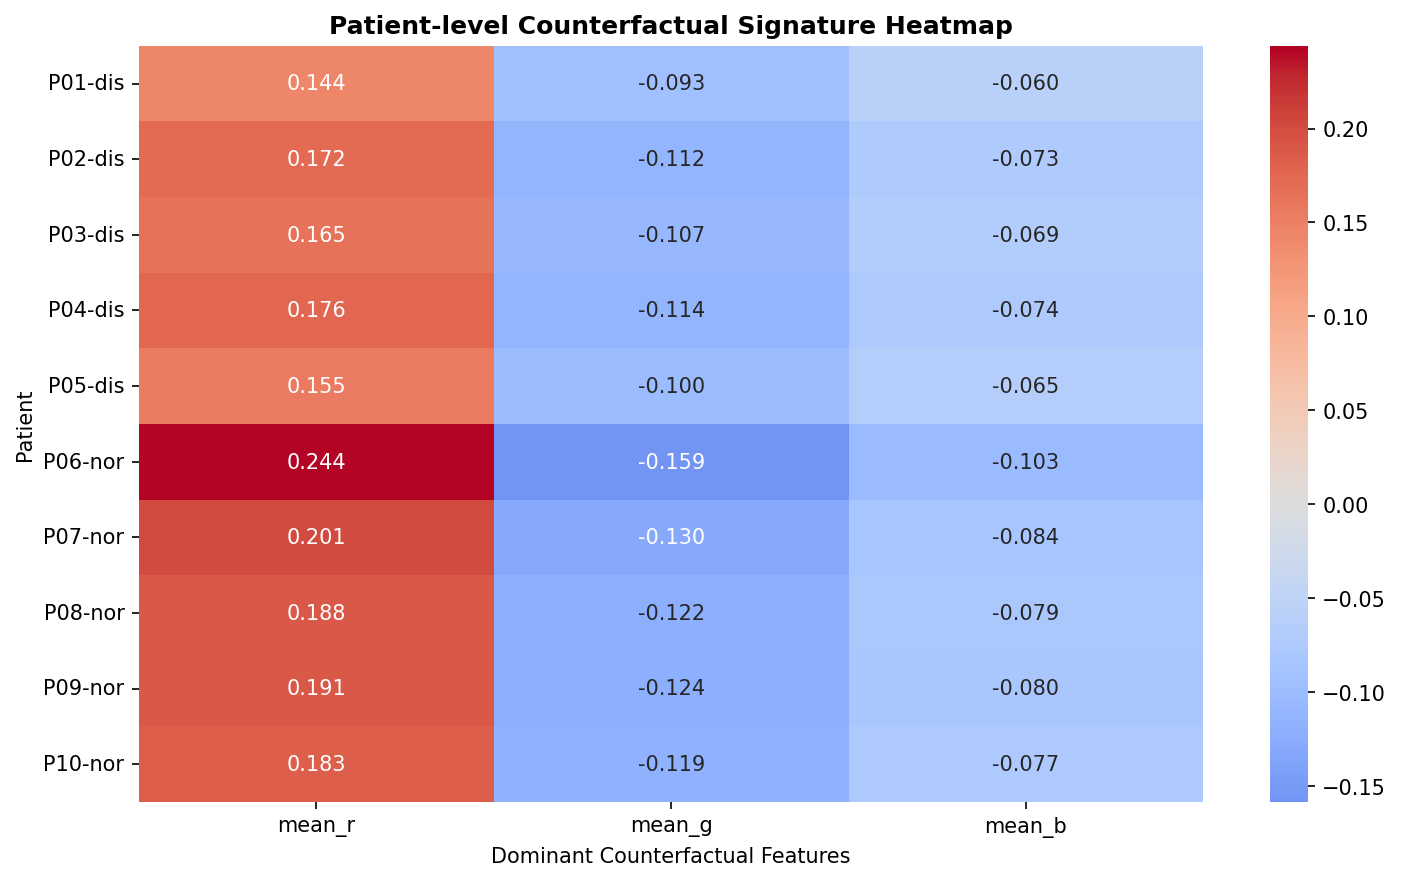
\includegraphics[width=0.92\textwidth]{plasmaxai_patient_heatmap.png}
\caption{Patient-level counterfactual signature heatmap summarizing disease-associated morphology patterns.}
\label{fig:heatmap}
\end{figure}
Figure~\ref{fig:heatmap} provides a compact patient-wise view of the counterfactual morphology pattern learned by the framework.

Taken together, the results position PlasmaXAI as a strong explainable classifier for plasma cell recognition. Its practical advantage is not only improved classification, but also transparent behavior through counterfactual features, uncertainty summaries, and patient-level consistency analysis.
\FloatBarrier

\section{Conclusion}
This paper presents PlasmaXAI as an explainable fusion framework for malignant plasma cell recognition. PlasmaXAI integrates deep image embeddings, morphology descriptors, and counterfactual reasoning into a unified decision path and achieves strong held-out performance while preserving interpretability. The model outperforms key baselines, shows meaningful sensitivity to removal of the counterfactual branch, and provides transparent diagnostic figures that support auditing and clinician-in-the-loop validation. The main limitation is the lack of external patient-level validation. Future work should focus on broader hematopathology cohorts, stain-robust generalization, and prospective clinical evaluation.

\begin{thebibliography}{99}
\bibitem{mmreview} Rajkumar, S.V.: Multiple myeloma: 2022 update on diagnosis, risk-stratification, and management. Am. J. Hematol. 97, 1086--1107 (2022)
\bibitem{litjens} Litjens, G., Kooi, T., Bejnordi, B.E., et al.: A survey on deep learning in medical image analysis. Med. Image Anal. 42, 60--88 (2017)
\bibitem{bera} Bera, K., Schalper, K.A., Rimm, D.L., Velcheti, V., Madabhushi, A.: Artificial intelligence in digital pathology---new tools for diagnosis and precision oncology. Nat. Rev. Clin. Oncol. 16, 703--715 (2019)
\bibitem{resnet} He, K., Zhang, X., Ren, S., Sun, J.: Deep residual learning for image recognition. In: Proceedings of the IEEE Conference on Computer Vision and Pattern Recognition, pp. 770--778 (2016)
\bibitem{densenet} Huang, G., Liu, Z., van der Maaten, L., Weinberger, K.Q.: Densely connected convolutional networks. In: Proceedings of the IEEE Conference on Computer Vision and Pattern Recognition, pp. 4700--4708 (2017)
\bibitem{wachter} Wachter, S., Mittelstadt, B., Russell, C.: Counterfactual explanations without opening the black box: Automated decisions and the GDPR. Harv. J. Law Technol. 31(2), 841--887 (2018)
\bibitem{diceml} Mothilal, R.K., Sharma, A., Tan, C.: Explaining machine learning classifiers through diverse counterfactual explanations. In: FAT* 2020, pp. 607--617 (2020)
\bibitem{calibration} Guo, C., Pleiss, G., Sun, Y., Weinberger, K.Q.: On calibration of modern neural networks. In: Proceedings of the 34th International Conference on Machine Learning, pp. 1321--1330 (2017)
\bibitem{unet} Ronneberger, O., Fischer, P., Brox, T.: U-Net: Convolutional networks for biomedical image segmentation. In: MICCAI 2015. LNCS, vol. 9351, pp. 234--241. Springer, Cham (2015)
\bibitem{attentionunet} Oktay, O., Schlemper, J., Folgoc, L.L., et al.: Attention U-Net: Learning where to look for the pancreas. arXiv preprint arXiv:1804.03999 (2018)
\bibitem{janowczyk} Janowczyk, A., Madabhushi, A.: Deep learning for digital pathology image analysis: A comprehensive tutorial with selected use cases. J. Pathol. Inform. 7, 29 (2016)
\bibitem{campanella} Campanella, G., Hanna, M.G., Geneslaw, L., et al.: Clinical-grade computational pathology using weakly supervised deep learning on whole slide images. Nat. Med. 25, 1301--1309 (2019)
\bibitem{lime} Ribeiro, M.T., Singh, S., Guestrin, C.: "Why should I trust you?": Explaining the predictions of any classifier. In: Proceedings of the 22nd ACM SIGKDD International Conference on Knowledge Discovery and Data Mining, pp. 1135--1144 (2016)
\bibitem{gradcam} Selvaraju, R.R., Cogswell, M., Das, A., et al.: Grad-CAM: Visual explanations from deep networks via gradient-based localization. In: Proceedings of the IEEE International Conference on Computer Vision, pp. 618--626 (2017)
\bibitem{shap} Lundberg, S.M., Lee, S.-I.: A unified approach to interpreting model predictions. In: Advances in Neural Information Processing Systems, pp. 4765--4774 (2017)
\end{thebibliography}

\end{document}
